\documentclass[../main.tex]{subfiles}

\begin{document}


\practica{8}{\emph{Bootloaders} y actualizaciones automáticas}

    \subsection{Objetivos}
        \begin{itemize}
            \item Entender el concepto de \emph{bootloader} y programar uno.
            \item Aprender a comunicar con un módulo WiFi externo a la placa para la descarga de aplicaciones.
            \item Comprender los pasos a seguir para ceder el control de una aplicación a otra.
            \item Aprender cómo compilar las aplicaciones para que convivan con el \emph{bootloader}.
        \end{itemize}

    \subsection{Fundamentos teóricos}

        Hacer aplicaciones perfectas a la primera es algo muy complicado. Aún habiéndolas hecho, normalmente se requieren actualizaciones a lo largo del tiempo. Una vez hemos fabricado un dispositivo y está operativo, el enlace de depuración se suele perder, así que se requieren métodos más sofisticados para reprogramarlo. Uno de los más extendidos es el de programar un pequeño \emph{bootloader}, o cargador, que se encarga además de actualizar el código principal si es necesario. En esta práctica programaremos un \emph{bootloader} capaz de descargar aplicaciones via Wifi, grabarlas en la Flash, y por último cederles el control. Aprenderemos además cómo tenemos que compilar nuestras aplicaciones para que el \emph{bootloader} las pueda cargar.


        El \emph{bootloader} es el primer programa que comienza a ejecutarse dentro del procesador. Su tarea, habitualmente, es realizar ciertas configuraciones iniciales, para posteriormente ceder el control a otro programa. Por ejemplo, en un ordenador ``estándar'', el \emph{bootloader} suele comprobar que los diferentes dispositivos están conectados correctamente y funcionando (tarjetas gráficas, memorias, pantalla, teclado, discos, etc), para posteriormente buscar distintos medios de arranque (USB, CD, Disco duro) y elegir automáticamente, o dar al usuario la opción, el modo de arranque del sistema.

        Es desde este \emph{bootloader} que uno puede configurar ciertos parámetros de muy bajo nivel del ordenador. Por ejemplo, encriptación de los discos (previa a la ejecución del sistema operativo), encendido automático a través de red, velocidad de los ventiladores\dots

        Una vez se han realizado todas estas configuraciones y comprobaciones, el \emph{bootloader} cede el control, generalmente, al sistema operativo (aunque en ocasiones hay varios niveles de \emph{bootloading}). Éste ya gestionará el resto de tareas para su ejecución simultánea, gestionando los recursos del sistema.

        En nuestro caso, no hay sistema operativo (aún), así que el bootloader simplemente cargará un programa sencillo. Para hacer algo más cercano a la realidad, haremos que nuestro \emph{bootloader}, previo a la carga del programa, lo descargue automáticamente de un servidor si es que no estuviera ya en la memoria del procesador. Así imitaremos, en cierta forma, la capacidad de muchos dispositivos empotrados de actualizarse automáticamente, sin necesidad de ser configurados por los puertos de depuración.

        Comprobará si la aplicación está ya instalada. De ser así, la lanzará directamente. Si no está, intentará descargarla de un servidor que configuraremos, por ejemplo, en nuestro teléfono. También daremos la opción de borrar la memoria donde alojaremos el programa, para poder probar el proceso varias veces sin necesidad de reprogramar la placa. El flujo de ejecución será el siguiente:

        \begin{enumerate}
            \item El procesador, desde su memoria de configuración, carga la dirección de arranque, en este caso la \MEMORY{0x20000} \REFMAN[1.9]. Nótese que esa dirección es un alias a la que nosotros utilizamos \MEMORY{0x08000000} \REFMAN[3.3.1], ya que la \PER{FLASH} se puede acceder desde dos rangos de direcciones diferentes. \footnote{Existe adicionalmente la posibilidad de programar dos direcciones diferentes de arranque, y controlar con un botón cuál de las dos se utiliza. Por defecto, la dirección de arranque será la de nuestro programa (\emph{bootloader} en este caso), y en la otra, se encuentra otro \emph{bootloader} diferente preprogramado por ST \REFMAN[1.9]. Para ver más detalles del \emph{bootloader} de ST consultar \ANMAN}
            \item El \emph{bootloader} se encuentra allí, situado al principio de la flash \MEMORY{0x08000000} (memoria de arranque) y toma el control.
            \item Si no hacemos nada, el \emph{bootloader} consulta la dirección objetivo del programa (\MEMORY{0x08010000}) y verifica si existe un programa. En ese caso salta a ejecutarlo.
            \item Si pulsamos un botón, el \emph{bootloader} entrará en modo actualización, e intentará conectarse a internet para descargar, flashear, y por último ejecutar nuestra aplicación.
            \item Si lo pulsamos aún más tiempo, borrará el contenido de la flash en la dirección \MEMORY{0x8010000}.
        \end{enumerate}

        \begin{figure}
            \centering
            \begin{tikzpicture}[
                node distance=1.5cm and 2cm,
                auto,
                >=stealth',
                % Estilos de los bloques
                startstop/.style={rectangle, rounded corners, draw=blue!80, fill=blue!10, thick, minimum width=3.5cm, minimum height=1cm, align=center},
                process/.style={rectangle, draw=gray!80, fill=gray!10, thick, minimum width=3.5cm, minimum height=1cm, align=center},
                decision/.style={diamond, aspect=2, draw=orange!80, fill=orange!10, thick, align=center, inner sep=2pt},
                action/.style={rectangle, rounded corners=2pt, draw=green!60!black, fill=green!10, thick, minimum width=3.5cm, minimum height=1.2cm, align=center},
                erase/.style={rectangle, rounded corners=2pt, draw=red!80, fill=red!10, thick, minimum width=3.5cm, minimum height=1cm, align=center}
            ]

                % Nodos principales (Columna Central)
                \node (start) [startstop] {\textbf{Arranque del Procesador}\\ \small Carga dir. \texttt{0x20000} (\texttt{0x08000000})};
                \node (bootloader) [process, below=of start] {\textbf{Control del Bootloader}\\ \small Ubicado en Flash (\texttt{0x08000000})};
                \node (button) [decision, below=1.8cm of bootloader] {\textbf{Estado del Botón}};

                % Rama Izquierda: Sin Pulsar
                \node (check) [decision, left=2.2cm of button] {¿Existe App?\\ \small en \texttt{0x08010000}};
                \node (run_app) [action, below=2cm of check] {\textbf{Ejecutar Aplicación}\\ \small Salto a \texttt{0x08010000}};

                % Rama Central: Pulsación Corta
                \node (update) [action, below=2cm of button] {\textbf{Modo Actualización}\\ \small Conectar a servidor/móvil $\rightarrow$\\ Descargar $\rightarrow$ Flashear};

                % Rama Derecha: Pulsación Larga
                \node (erase) [erase, right=2.2cm of button] {\textbf{Borrar Memoria}\\ \small Limpiar Flash \\ \texttt{0x08010000}};

                % Conexiones secuenciales
                \draw [->, thick] (start) -- (bootloader);
                \draw [->, thick] (bootloader) -- (button);

                % Transiciones del Botón
                \draw [->, thick] (button) -- node[above, font=\small] {Sin pulsar} (check);
                \draw [->, thick] (button) -- node[right, font=\small] {Pulsación corta} (update);
                \draw [->, thick] (button) -- node[above, font=\small] {Pulsación larga} (erase);

                % Lógica de Comprobación y Ejecución
                \draw [->, thick] (check) -- node[right, font=\small] {Sí} (run_app);
                \draw [->, thick] (check.south east) -- node[below left, font=\small] {No} (update.north west);
                \draw [->, thick] (update) -- (run_app);
            \end{tikzpicture}
            \caption{Secuencia de arranque de nuestra aplicación}
            \label{fig:bootloader_sequence}
        \end{figure}

        Cuando un \emph{bootloader} cede el control, no puede hacerlo de cualquier manera. Debe asegurarse de que entrega el procesador a la aplicación invitada en un estado inicial aceptable. Por ejemplo, deberá desactivar interrupciones, configurar correctamente la pila, e indicar la nueva dirección de inicio de programa al procesador. Un fallo en cualquiera de estos pasos podría suponer que el programa cargado no llegue a funcionar, generalmente porque empiece a ejecutarse en zonas de memoria restringidas.

        Por otro lado, las aplicaciones también deben estar preparadas para su correcta ejecución. Normalmente, al preparar una aplicación ``usual'' en un procesador \emph{bare-metal} como el nuestro, la compilamos con las opciones por defecto y esto es suficiente, ya que se ejecuta desde la dirección inicial de ejecución del procesador. Pero en este caso, en esa dirección tenemos el \emph{bootloader}. Por tanto, debemos compilarla con la dirección de inicio objetivo en la cual la vaya a cargar el \emph{bootloader}, asegurando así un correcto funcionamiento. 

        \subsubsection{El módulo Wifi ESP-01S}

            Nuestro procesador no tiene manera de realizar comunicación inalámbrica, por tanto se utiliza un módulo externo \texttt{ESP-01S}. Este módulo permite, a través de una comunicación \PER{UART} desde el procesador \MCU, establecer una conexión WiFi y enviar o recibir datos a través de protocolos como \texttt{HTTP} y \texttt{TCP}, que serán vistos desde nuestra aplicación a través de la \PER{UART}. 

            Nosotros lo veremos solo como usarios y con un conjunto reducido de comandos. Puedes consultar la documentación completa en \url{https://espressif-docs.readthedocs-hosted.com/projects/esp-at/en/release-v2.2.0.0_esp8266/AT_Command_Set/index.html}.
       

    \subsection{Desarrollo de la práctica}

        \subsubsection{Configuración previa al \emph{bootloader}}

            Como hemos visto anteriormente, la idea es hacer un \emph{bootloader} con diversas opciones (descargar app, ejecutar, borrar) que se seleccionarán de manera semi-automática en función del estado de la memoria, y el de un botón que podremos pulsar más o menos tiempo.

            Para medir el tiempo, vamos a hacer uso de un periférico que hasta ahora no habíamos utilizado, el \PER{SysTick} \PMMAN[4.4]. Este periférico se utiliza para llevar una cuenta de los \emph{ticks} que han pasado en el procesador. La cuenta de \emph{tick} se incrementa cada cierto tiempo, dependiente de la velocidad del reloj (16MHz por defecto) y la configuración del periférico. Por ejemplo, podemos configurarlo para que cuente cada milisegundo. Así, podremos consultar en cualquier momento el valor de \emph{tick} actual para saber cuánto tiempo ha pasado desde otro momento en el que realizáramos otra consulta. El código necesario se incluye a continuación:

            \begin{lstlisting}
                #define SYSTICK_BASE_ADDR  		(0xE000E010UL)

                typedef struct {
                    volatile uint32_t CTRL;     // 0x00
                    volatile uint32_t LOAD;     // 0x04
                    volatile uint32_t VAL;      // 0x08
                    volatile uint32_t CALIB;    // 0x0C
                } SysTick_TypeDef;

                #define SysTick           	((SysTick_TypeDef *) SYSTICK_BASE_ADDR)

                volatile uint32_t msTicks = 0;
                void SysTick_Handler(void) {
                    msTicks++;
                }

                void SysTick_Init(void) {
                    // Default HSI clock is 16MHz on reset. 1ms tick = 16,000 cycles.
                    SysTick->LOAD = (16000U - 1U);
                    SysTick->VAL  = 0U;
                    SysTick->CTRL = (1U << 2) | (1U << 1) | (1U << 0); // Processor Clock, Int Enable, Enable
                }

                void SysTick_Disable(void) {
                    SysTick->LOAD = 0U;
                    SysTick->VAL  = 0U;
                    SysTick->CTRL = 0U;
                }

                uint32_t GetTick(void) {
                    return msTicks;
                }

                void Delay_ms(uint32_t ms) {
                    uint32_t start = GetTick();
                    while ((GetTick() - start) < ms);
                }
            \end{lstlisting}

            Por otro lado, necesitamos configurar los periféricos a utilizar por nuestro bootloader. Estos son:

            \begin{itemize}
                \item El botón de usuario.
                \item La \PER{UART} de depuración (ya configurada en prácticas anteriores)
                \item La \PER{UART} de comunicación con el ESP-01S
            \end{itemize}

            Se proporcionan las siguientes funciones ya hechas para ello:

            \begin{lstlisting}
                void Peripherals_Init(void) {
                    // Enable USARTs and their GPIOs
                    RCC_AHB1ENR->bits.GPIOCEN = 1;
                    RCC_AHB1ENR->bits.GPIODEN = 1;
                    RCC_APB1ENR->bits.USART5EN = 1;	// comm with espressif
                    RCC_APB2ENR->bits.USART6EN = 1; // comm with computer (stlink)

                    /* --- USART6 Pin Configuration (ST-LINK VCP: PC6=TX, PC7=RX) --- */
                    GPIO_CONFIG(GPIOC, 6, GPIO_MODE_ALT, GPIO_OTYPE_PP, GPIO_OSPEED_HIGH, GPIO_PUPD_PU, GPIO_AF8_USART6);
                    GPIO_CONFIG(GPIOC, 7, GPIO_MODE_ALT, GPIO_OTYPE_PP, GPIO_OSPEED_HIGH, GPIO_PUPD_PU, GPIO_AF8_USART6);

                    /* --- UART5 Pin Configuration (ESP8266: PC12=TX, PD2=RX) --- */
                    GPIO_CONFIG(GPIOC, 12, GPIO_MODE_ALT, GPIO_OTYPE_PP, GPIO_OSPEED_HIGH, GPIO_PUPD_PU, GPIO_AF8_USART5);
                    GPIO_CONFIG(GPIOD,  2, GPIO_MODE_ALT, GPIO_OTYPE_PP, GPIO_OSPEED_HIGH, GPIO_PUPD_PU, GPIO_AF8_USART5);

                    /* --- Baud Rate Setup ---
                    * Default HSI Clock = 16 MHz. Target Baud Rate = 115200.
                    * USARTDIV = 16,000,000 / 115200 = 138.88 => BRR = 139 (0x8B)
                    */
                    UART_BRR_SET(USART6, 139);
                    UART_BRR_SET(UART5, 139);
                    // enable UARTS + TX + RX
                    UART_ENABLE_SET(USART6, 1);
                    UART_TX_MODE_SET(USART6, 1);
                    UART_RX_MODE_SET(USART6, 1);
                    UART_ENABLE_SET(UART5, 1);
                    UART_TX_MODE_SET(UART5, 1);
                    UART_RX_MODE_SET(UART5, 1);
                }

                void UserButton_Init(void) {
                    RCC_AHB1ENR->bits.GPIOAEN = 1;
                    GPIO_CONFIG(GPIOA, 0, GPIO_MODE_INPUT, GPIO_OTYPE_PP, GPIO_OSPEED_LOW, GPIO_PUPD_PD, 0);
                }
            \end{lstlisting}

        \subsubsection{Cesión del control a la aplicación}

            Para poder ceder el control a la aplicación, debemos hacer dos cosas. En primer lugar, ser capaces de comprobar que la aplicación existe y está descargada en la memoria. En segundo, cambiar el control del procesador a esa zona de memoria para su ejecución.

            Comenzamos con la comprobación de existencia. Las aplicaciones, al compilarse, tienen una estructura muy concreta que se genera a partir del \emph{Linker Script}. Este fichero (\texttt{STM32F723IEKX\_FLASH.ld}), que viene creado ya de manera automática con nuestros proyectos (aunque podemos customizarlo), tiene esta pinta (se destacan aquí solo algunas partes):

            \begin{lstlisting}
                // Punto de entrada del código al comenzar a ejecutarse
                // Esta función llama luego a main
                ENTRY(Reset_Handler)

                // posición en memoria de la pila, justo al final de la memoria RAM
                _estack = ORIGIN(RAM) + LENGTH(RAM); 

                // tamaños mínimos de pila y montón. Si no caben (por ser muy
                // grande el programa), la compilación fallará
                _Min_Heap_Size = 0x200;  
                _Min_Stack_Size = 0x400;

                // direcciones, permisos y tamaño de las memorias
                // importante que en la flash no se tienen permisos
                // de escritura (por defecto)
                MEMORY
                {
                    RAM    (xrw)    : ORIGIN = 0x20000000,   LENGTH = 256K
                    FLASH   (rx)    : ORIGIN = 0x8000000,   LENGTH = 512K
                }

                // aquí comienzan a colocarse los ``trozos'' de programa
                SECTIONS
                {
                    // primero una tabla de vectores con diferentes direcciones 
                    // para las distintas interrupciones del sistema
                    .isr_vector :
                    {
                        . = ALIGN(4);
                        KEEP(*(.isr_vector)) /* Startup code */
                        . = ALIGN(4);
                    } >FLASH

                    // luego se coloca el código
                    .text :
                    {
                        . = ALIGN(4);
                        *(.text)           /* .text sections (code) */

                    // continúa (ver archivo de referencia en cualquier proyecto)
                    // .................
            \end{lstlisting}

            Este linker script gobierna cómo el código se ordena y coloca en el binario final. Básicamente, va colocando todos los símbolos (por símbolo se entienden variables, funciones, etc) uno detrás de otro. Los símbolos se definen desde el código, al definir funciones o usar variables. Aunque nosotros no lo hacemos a mano, cada vez que definimos una función, se crean símbolos que comienzan por \texttt{.text}, o cada vez que definimos variables, símbolos que comienzan por \texttt{.data}. Eso es lo que coloca el linker posteriormente y de manera ordenada.

            Ciertos símbolos especiales, como el código primero que se ejecuta, se definen desde el fichero \texttt{startup\_stm32f723iekx.s} (ya creado por defecto con cualquier proyecto). Aquí tenemos la función \texttt{Reset\_Handler} que será la primera ejecutada al lanzar cualquier programa:

            \begin{lstlisting}
                .section .text.Reset_Handler
                .weak Reset_Handler
                .type Reset_Handler, %function
                Reset_Handler:
                ldr   r0, =_estack
                mov   sp, r0          /* set stack pointer */
              
                // ... inicialización de diferentes secciones de memoria
                // salto a la función principal.
                bl main
            \end{lstlisting}

            Y cómo sabe el procesador que tiene que llegar aquí al iniciar? Miremos en otra zona del código de inicialización:

            \begin{lstlisting}
                .section .isr_vector,"a",%progbits
                .type g_pfnVectors, %object

                g_pfnVectors:
                .word _estack
                .word Reset_Handler
                // ... punteros a interrupciones
            \end{lstlisting}

            Es decir, si nos fijamos en el contenido \texttt{SECTIONS} de nuestro \emph{linker script}, veremos que lo primero que coloca en el binario es \texttt{.isr\_vector}. A su vez, esta sección tiene, en primer lugar, el valor inicial de la pila, y la dirección de comienzo \texttt{Reset\_Handler}. El procesador ya es conocedor de esto \PMMAN[2.1.3] y cargará ambos al resetearse.

            Se ofrece a modo ilustrativo esta visualización del espacio de memoria de nuestra aplicación, construido desde el linker script y el código de inicialización:

            % Custom Color Palette
            \definecolor{HeaderDark}{HTML}{1F4E78}
            \definecolor{VectorBlue}{HTML}{D9E1F2}
            \definecolor{CodeBlue}{HTML}{BDD7EE}
            \definecolor{RoDataBlue}{HTML}{DEEBF7}
            \definecolor{InitBlue}{HTML}{E9EEF4}
            \definecolor{DataGreen}{HTML}{E2EFDA}
            \definecolor{BssGreen}{HTML}{C6E0B4}
            \definecolor{HeapOrange}{HTML}{FCE4D6}
            \definecolor{StackOrange}{HTML}{F8CBAD}
            \definecolor{ReservedGray}{HTML}{F2F2F2}

            \newcolumntype{C}{>{\centering\arraybackslash}X}
            \newcolumntype{L}{>{\raggedright\arraybackslash}X}

            \begin{tabularx}{\textwidth}{|>{\ttfamily}p{2cm}|>{\ttfamily}p{2.8cm}|X|}
                \hline
                \rowcolor{HeaderDark}
                \color{white}Address (Flash) & \color{white}Contents & \color{white}Description\\ \hline
                \rowcolor{VectorBlue}
                0x08000000 & .isr\_vector & Vector Table: Initial SP, Reset\_Handler, ISR Handlers  \\ \hline
                \rowcolor{StackOrange}
                0x08000000 & \_estack (0x20040000) & Initial Stack Pointer Value (Top of RAM) \\ \hline
                \rowcolor{CodeBlue}
                0x08000004 & Reset\_Handler & Initial Execution Entry Address (Reset Vector) \\ \hline
                \rowcolor{VectorBlue}
                0x08000008 & NMI\_Handler & Non-Maskable Interrupt Handler \\ \hline
                \rowcolor{VectorBlue}
                0x0800000C & HardFault\_Handler & Hardware Fault Exception Handler \\ \hline
                \rowcolor{VectorBlue}
                0x08000010+ & Core Exceptions & MemManage, BusFault, UsageFault, SVC, SysTick \\ \hline
                \rowcolor{VectorBlue}
                0x08000040+ & Peripheral IRQs & WWDG, PVD, RTC, Flash, RCC, EXTI, DMA, TIM, etc. \\ \hline
                \rowcolor{CodeBlue}
                0x08000... & .text & Executable Program Code \\ \hline
                \rowcolor{RoDataBlue}
                ... & .rodata & Constant Data, String Literals, Read-Only Variables \\ \hline
                \rowcolor{RoDataBlue}
                ... & .data & Initialized global variables  \\ \hline
                \rowcolor{InitBlue}
                ... & ... & Various code utilities  \\ \hline
                \rowcolor{HeaderDark}
                \color{white}Address (RAM) & \color{white}Contents & \color{white}Description \\ \hline
                \rowcolor{DataGreen}
                0x20000000 & .data & Initialized Global/Static Data (Copied from Flash) \\ \hline
                \rowcolor{BssGreen}
                ... & .bss & Uninitialized Global Data (Zero-filled by startup) \\ \hline
                \rowcolor{HeapOrange}
                ... & Dynamic Heap & Minimum Reserved Size: 0x200 (512 Bytes) $\uparrow$ Grows Up \\ \hline
                \rowcolor{ReservedGray}
                ... & Unallocated & Available RAM for Dynamic Stack/Heap Overlap \\ \hline
                \rowcolor{StackOrange}
                0x2003FC00 & Main Stack & Minimum Reserved Size: 0x400 (1024 Bytes) $\downarrow$ Grows Down \\ \hline
                \rowcolor{StackOrange}
                0x20040000 & \_estack  & Highest Stack Address (End of RAM) \\ \hline
            \end{tabularx}

            Observamos que, como habíamos dicho, el primer valor que se encuentra en nuestro programa, en \MEMORY{0x08000000} es la dirección de la pila, para a continuación tener en \MEMORY{0x08000004} la dirección inicial a la que saltar (es decir, un puntero). Así pues, si en una dirección de memoria encontramos esta estructura, o similar, podemos asumir que en ese lugar tenemos un programa guardado. Nuestra función de comprobación de existencia de programa puede ser, por ejemplo, la siguiente:

            \begin{lstlisting}
                //Check for app presence at a given location
                uint8_t IsApplicationValid(uint32_t address) {
                    uint32_t sp = *(volatile uint32_t *)address;

                    // Check if initial Stack Pointer points into valid SRAM range (0x200XXXXX)
                    if ((sp & 0x2FF00000) == 0x20000000) {
                        return 1;
                    }
                    return 0;
                }
            \end{lstlisting}

            Ahora, una vez detectada una aplicación en una ubicación concreta de memoria, debemos conseguir saltar a ella. Lo más importante en este punto es saber que tenemos que dejar el procesador en un estado totalmente neutro, ya que de lo contrario, la nueva aplicación podría sufrir comportamientos inesperados. Imaginemos por ejemplo que no desactivamos las interrupciones o ciertos periféricos: el procesador seguiría ejecutando funcionalidad totalmente ajena a nuestra aplicación.

            Por tanto, lo primero es desactivar cualquier cosa que hayamos utilizado. En nuestro caso, el \emph{ticker} del sistema y los periféricos \PER{GPIO} y \PER{UART}. 

            \begin{lstlisting}
                void JumpToApplication(uint32_t address) {
                    // Disable any active interrupts (only SysTick in our case)
                    SysTick_Disable();

                    // Disable the peripherals we were using
                    RCC_AHB1ENR->bits.GPIOAEN = 1;
                    RCC_AHB1ENR->bits.GPIOCEN = 1;
                    RCC_AHB1ENR->bits.GPIODEN = 1;
                    RCC_APB1ENR->bits.USART5EN = 1;	// comm with espressif
                    RCC_APB2ENR->bits.USART6EN = 1; // comm with computer (stlink)
            \end{lstlisting}

            Por otro lado, tenemos que reubicar también el puntero de la pila para que se ubique al principio del nuevo rango requerido. De lo contrario, estaríamos trabajando con la pila en direcciones de memoria desconocidas, lo cual puede traer fallos de acceso a memoria o, aún peor, sobreescribir nuestro nuevo código si hubiera solape. El valor inicial del \REG{SP} se extrae de la dirección inicial del programa:

            \begin{lstlisting}
                    // Set Main Stack Pointer (MSP)
                    __asm volatile ("msr msp, %0" : : "r" (*(volatile uint32_t *)address) : );
            \end{lstlisting}

            Ahora ya está todo listo para saltar a la función inicial (que recordemos es el \texttt{Reset\_Handler} del archivo de inicialización \texttt{startup\_stm32f723iekx.s}). Como su dirección inicial se encuentra en la segunda palabra del binario (\texttt{address + 4}), la extraemos de ahí, y la convertimos a un tipo de función \texttt{void} antes de llamarla.

            \begin{lstlisting}
                    // Branch to reset handler of target firmware
                    typedef void (*pFunction)(void);
                    uint32_t JumpAddress = *(volatile uint32_t *)(address + 4);
                    pFunction JumpToApp = (pFunction)JumpAddress;
                    JumpToApp();
                }
            \end{lstlisting}

            A partir de aquí, habremos perdido completamente el control del programa, y toda la ejecución queda a merced de la aplicación objetivo.

        \subsubsection{La memoria Flash}

            Nuestro código se almacenará en la memoria Flash del procesador. Esta memoria tiene la capacidad, al contrario de la RAM, de retener el contenido incluso tras apagarse y encenderse el procesador. Sin embargo, su uso por el programador está restringido (básicamente para evitar accidentalmente sobreescribir el código) así que tenemos que permitir los accesos en ella si queremos hacerlo. Echa un vistazo a la documentación de la \PER{FLASH} en \REFMAN[3.7.2] y completa el código de desbloqueo de la flash:

            \begin{lstlisting}
                /* Flash Keys */
                #define FLASH_KEY1        0x45670123U
                #define FLASH_KEY2        0xCDEF89ABU
                void Flash_Unlock(void) {
                    // ... completar si la flash está bloqueada (CR)
                    // ... desbloquear con la secuencia de claves en KEYR
                }
            \end{lstlisting}

            Observa también la función \texttt{ESP01S\_DownloadAndFlash} y verás que el flujo de programación es, a grandes rasgos, el siguiente:

            \begin{lstlisting}
                Flash_Unlock();
                Flash_ClearErrors();
                for (bytes to write)
                    Flash_WriteByteRaw(current_flash_addr++, byte);
                Flash_Lock();
            \end{lstlisting}

            Es decir, nos aseguramos de que la protección de la flash solo se quita en el fragmento de código que flashea el binario descargado, y en ningún otro sitio, para evitar errores.

        \subsubsection{Programación del \emph{bootloader}}

            Ahora, con el archivo descargado y las funciones auxiliares de salto a programa, debemos programar el \emph{bootloader}. Básicamente vamos a crear un código \texttt{main.c} que ceda el control a una región de memoria específica (en concreto, la \MEMORY{0x08010000} como vimos anteriormente). Completa el siguiente código para ello, añadiendo además los mensajes de depuración (Ver práctica 3) que consideres oportunos. Utiliza todas las funciones programadas anteriormente.

            \begin{lstlisting}
                int main(void) {
                    // ... completar 
                    // ... inicializar systick, periféricos y botón de usuario

                    uint8_t app_valid = IsApplicationValid(ADDR_FLASH_SECTOR_4);
                    uint8_t button_pressed = GPIO_PIN_READ(GPIOA, 0);
                    // Boot decision
                    // ... completar
                    // ... si el botón no está pulsado, comprobar si la app es válida y saltar a ella
                    // ... si el botón está pulsado, comprobar de nuevo tras 2 segunods
                    // ... si sigue pulsado, en ese caso borrar la flash
                    // ... en cualquier otro caso, continuar con la descarga de la app


                    // Initialize ESP8266 device
                    if (!ESP01S_Init()) {
                        while (1);
                    }

                    // Connect Wi-Fi
                    if (!ESP01S_ConnectWiFi()) {
                        while (1);
                    }

                    // We must erase before flashing new stuff, since bits only
                    // change from 1 to 0 and not vice versa when flashing.
                    // This ensures initial state is 0xffffffff
                    Flash_EraseSector(FLASH_TARGET_SECTOR);

                    // Download over TCP and Flash directly
                    if (!ESP01S_DownloadAndFlash()) {
                        while (1);    
                    }

                    JumpToApplication(ADDR_FLASH_SECTOR_4);
                }
            \end{lstlisting}


        \subsubsection{Compilación de la aplicación}

            Con esta práctica se proporciona un fichero binario compilado de ejemplo. No obstante, si queremos compilar el nuestro propio (con otro programa) tenemos que seguir unos pasos para asegurar que funcione.

            Lo primero es ceder el control completamente de forma correcta. Hasta ahora, lo ``único'' que hemos hecho ha sido saltar a la dirección de la función inicial \texttt{Reset\_Handler} de la aplicación objetivo. Pero, y todas las interrupciones? Si ahora activásemos una interrupción, saltaría a la tabla de interrupciones de la aplicación original, fallando por completo el código. Como vimos anteriormente, la aplicación tiene al comienzo una tabla de vectores que indican las direcciones de memoria de las diferentes interrupciones y código de arranque. El Bloque de Control del Sistema \PER{SCB} (\PMMAN[4.3]) guarda en su registro \REG{VTOR} la dirección inicial de dicha tabla (es decir, la dirección inicial de nuestro código). Así pues, debemos cambiarla para reubicar todas las interrupciones de una sola tacada. Esto lo podemos hacer redefiniendo la función \texttt{System\_Init} (definida como \texttt{.weak} precisamente para que nosotros la redefinamos y le demos funcionalidad si es necesario).

            \begin{lstlisting}
                void SystemInit(void) {
                    SCB->VTOR = 0x08010000; 
                }
            \end{lstlisting}

            Por otro lado, tendremos que indicar en el linker script \texttt{STM32F723IEKX\_FLASH.ld} el cambio de dirección inicial:

            \begin{lstlisting}
                FLASH    (rx)    : ORIGIN = 0x8010000,   LENGTH = 256K
            \end{lstlisting}
            
            Finalmente, activamos la generación del archivo binario desde \texttt{C/C++ Build > Settings > MCU/MPU Post build outputs > Convert to binary file (-O binary)}.

            Al compilar, se nos generará ahora un archivo \texttt{.bin} que es el que habrá que flashear.


        \subsubsection{Configuración del servidor de descarga}

            Llegados a este punto, deberíamos tener un bootloader funcional que... no puede hacer nada pues no tiene un servidor al que conectarse. Necesitamos hacer dos cosas:

            \begin{enumerate}
                \item Asegurarnos de que el módulo ESP-01S está conectado a nuestra placa.
                \item Configurar un servidor para que se descargue el archivo binario.
            \end{enumerate}

            Lo primero es relativamente sencillo, simplemente hay que colocar el módulo en el conector CN14 que se encuentra en la placa (conector con 8 pines huecos), en la dirección que indica la marca blanca inferior.

            Respecto a lo segundo, se puede hacer de muchas maneras. La más cómoda es hacerlo desde nuestro propio teléfono, habilitando un punto inalámbrico que actúe como entrada a la red para nuestro programa. Asegúrate de configurar correctamente la conexión creando el archivo \texttt{ESP01S\_config.h}

            \begin{lstlisting}
                #define WIFI_SSID       "<nombre de tu red wifi>"
                #define WIFI_PASSWORD   "<password de tu red wifi>"
                #define SERVER_IP  	  	"<ip de tu servidor>"
                #define SERVER_PORT		<puerto de tu servidor>
                #define FILE_PATH      	"<nombre del fichero>"
            \end{lstlisting}

            Lo siguiente es abrir un servidor \texttt{http} en nuestro teléfono que sirva el binario \texttt{hello.bin} o cualquier otro que hayamos creado a mano.

            \begin{itemize}
                \item En Android, podemos hacerlo descargando la aplicación \texttt{SHTTPS} \url{https://play.google.com/store/apps/details?id=com.phlox.simpleserver&hl=es} y configurándola como vemos en la \Cref{fig:shttps}. Únicamente tendremos que iniciar el servidor, poner la \texttt{Root Folder} apuntando a donde tengamos guardado el archivo binario de la aplicación, y seleccionar la interfaz de nuestra red inalámbrica (normalmente llamada \texttt{ap\_XXX}) para que nos de la IP que tendremos que poner en la configuración anterior.
                
                    \begin{figure}
                        \centering
                        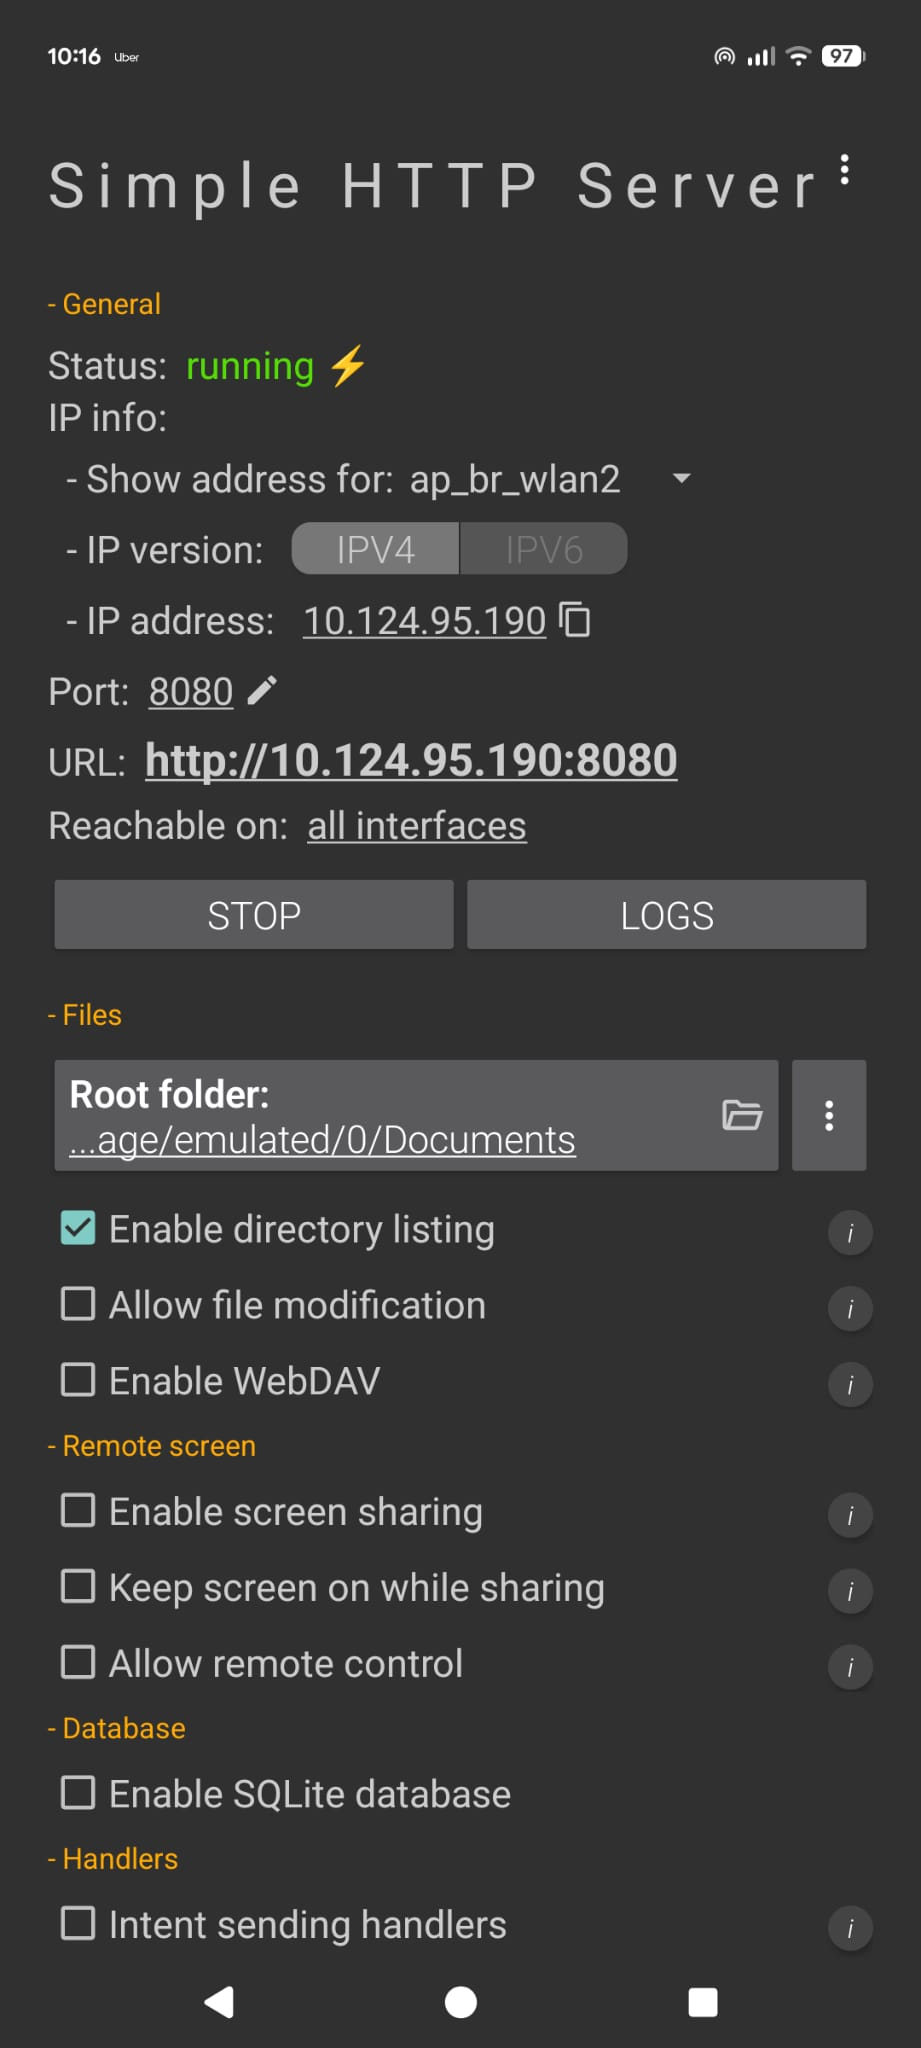
\includegraphics[width=0.5\textwidth]{res/shttps.jpeg}
                        \caption{Configuración SHTTPS Android}
                        \label{fig:shttps}
                    \end{figure}

                \item En IOS, hay aplicaciones similares como \url{https://apps.apple.com/es/app/simple-server-http-server/id6443893597} o \url{https://apps.apple.com/es/app/share-server/id6754194116}.
            \end{itemize}

            Y listo! Ahora nuestra aplicación debería ser capaz de conectarse al punto WiFi de nuestro teléfono, descargar el binario, flashearlo, y lanzarlo a ejecución! Asegúrate de poner mensajes de depuración si tienes problemas, para ver dónde pueda haber dificultades.

    \subsection{Para hacer más}

        En ocasiones, en lugar de tener una aplicación \emph{bootloader} que se encarga de descargar el binario actualizado, se fusionan ambas funcionalidades en una sola (\emph{bootloader} + app). Así, el propio \emph{bootloader} también es actualizado. Para ello, se reservan dos regiones de flash diferentes, $A$ y $B$. La aplicación $A$, cuando detecte una actualización (a través de WiFi por ejemplo), la escribirá en $B$, y configurará el procesador para arrancar desde ahí la próxima vez. Y viceversa, si la $B$ es la que está en juego, actualizará $A$. Así, incluso si durante el proceso de actualización fallara algo, siempre habrá una de las dos aplicaciones funcional. Investiga cómo se haría este proceso en nuestro procesador \MCU.

\end{document}